\chapter{Literature Review}

\section{Anomaly Detection}
\label{section:anomalyDetectionLiteratureReview}
\subsection{Overview}

% definition of anomaly detection
\textit{Anomaly detection} is a problem of finding patterns in data that do not follow expected normal behavior represented by the majority of the data points. It follows that defining normal behaviour is one of the crucial challenges of anomaly detection. The unusual patterns are also called \textit{outliers} or \textit{anomalies} and anomaly detection is referred to as \textit{outlier detection}. Outlier was defined by \cite{ORD1996175} as an outlying observation that appears to deviate markedly from other members of the sample in which it occurs. In other words, statistical properties of the anomalous data points are not in alignment with the rest of the data. Outliers vary depending on the domain and may arise due to various reasons, such as fraudulent behaviour in credit card fraud, intrusion in computer networks, system failures, mechanical faults in industrial applications, deviations caused by natural behaviour or human error. Initially, outliers would be detected manually by the hand of a domain expert. Nowadays, anomaly detection's focus is identifying anomalous behavior automatically. Anomaly detection is also related to \textit{noise}. Noise is defined as an unwanted phenomenon in data, which is not of interest to the analyst, but acts as a hindrance to data analysis \cite{cvbakv2009}. Noise is  caused by an external factor not related to the distribution that generates the data \cite{ggh2017} and leads to excessively complex models with deteriorated performance \cite{wu2007}. 

In our thesis we focus on anomaly detection in time series data. Time series outlier analysis examines anomalies in the behavior of the data across time \cite{gupta2014}. An outlier in time series data is a data point, which is not following a common behaviour, either a general long-term trend or a tendency of the data to increase or decrease in seasonal patterns. 

\todo{Type of anomalies}
%https://scholarworks.sjsu.edu/cgi/viewcontent.cgi?article=1640&context=etd_projects

% is dependant on the \textit{input data type}, \textit{outlier type} and the \textit{nature of the method} \cite{gcml2020}, which are described in the next section.

% definition of outlier
% examples where is AD used
% why is there interest in studying time series data
% anomaly detection in time series 
\\
We can classify anomaly detection methods into three broad categories: \textit{supervised}, \textit{semi-supervised} and \textit{unsupervised} anomaly detection. Supervised learning algorithms are trained by examples and require dataset, that is already labeled. On the other hand, unsupervised methods don't require labeled data at all. Semi-supervised methods combine both approaches by assuming that normal class instances are labeled.

% describe the advantages of unsupervised methods over supervised https://reader.elsevier.com/reader/sd/pii/S0167404818306333?token=9C7DC222C83AC3AD33CBF921C2E23508BEA68B59C5336EC0200EF02A1F60DAB2916EEE9D83663EE9029AB30B9C1CC538

\subsection{Supervised Anomaly Detection}
Supervised methods require pre-labelled data, where labels describe whether the behaviour in each data instance is normal or abnormal (anomalous). Then the main focus of supervised learning techniques is to derive a model from labeled data, which maximizes the discrimination between the classes (normal and anomalous). A drawback of supervised method is that it can be only trained on the types of anomalies, that have been introduced in the training examples. It cannot handle previously unseen anomalies. 

 \subsection{Semi-supervised Anomaly Detection}
 %https://www-users.cs.york.ac.uk/vicky/myPapers/Hodge+Austin_OutlierDetection_AIRE381.pdf
 %https://researchbank.swinburne.edu.au/file/cee84793-6f09-49ce-a099-41451c803b81/1/mostafa_farshchi_thesis.pdf
 Semi-supervised approaches assume that some portion of training data is labeled. Only labels for instances of normal class are provided, while labels for classes describing anomaly are not required. The rest of the data is unlabeled. Thus, in a semi-supervised mode, the model capturing normal behavior is built and used to identify anomalous behaviour. A class describing normal data is most commonly used primarily because it is more readily available, whereas labeled data set that would cover every anomaly is difficult to obtain.  \cite{anomalyDetectionSurvey}. 
 
\subsection{Unsupervised Anomaly Detection}
 Unsupervised learning, unlike supervised learning, doesn't require any prior knowledge of the data. One of the main difficulties that anomaly detection has to face is unlabeled data. In most cases, logs with labeled anomalies are not available. The log annotating process would have to be executed manually by the experts - developers familiar with the system. Along with the volume of data growth, labeling gets very time consuming. Due to this fact, in practice, anomaly detection relies mostly on unsupervised learning to deal with unlabeled data. Unsupervised anomaly detection algorithms learn what normal behavior looks like. Based on these observation, unsupervised method based systems detect anomalies as outliers, that significantly differ from other examples. In addition, any type of anomaly can be detected by these systems. Thus, the main difference between supervised and unsupervised learning techniques is that the former focus on discriminating concept classes, while the latter rather focus on data characterization \cite{Goernitz_2013}. % They work based on the observation that an abnormal instance usually manifests as an outlier point that is distant from other instances. As such, unsupervised learning techniques, such as clustering, can be applied.
 
 Because of the character of our data, for this research, we have used unsupervised methods for anomaly detection.
 
 \subsubsection{Isolation Forest}
 Isolation Forest or iForest \cite{liu2012isolation} is an ensemble approach to detect anomalies. Majority of existing model-based methods are trying to model normal behaviour, and then deviation from the normal region that does not fit the model well is considered an anomaly \cite{introToDataMining2005}. Isolation Forest approach, on the other hand, directly isolates anomalies without using the distance from the previously defined normal region. It is taking advantage of two properties that can be observed in anomalies. Anomalous instances are the minority data points and their attribute-values are very different from normal instances. Because of these properties, anomalies are susceptible to a concept called \textit{isolation} which is the main idea behind Isolation Forests. They defined isolation in their research paper as 'separating an instance from the rest of the instances'.\\
 Isolation Forest starts by selecting a random attribute and then creates a random partition between the maximum and minimum values of that attribute. This process is applied recursively until all samples are isolated, which can be represented by a binary tree structure (Isolation Tree of iTree). Then the number of partitions performed in order to isolate a point is equal to the length of the traversal path from the root node to a terminating node. The iForest is built by adding a given number of iTrees generated by randomly generating partitions and their averaged traversal path lengths are then used as an anomaly score measure. It is easy to see that isolating anomaly instances happens closer to the root of the tree, hence the lengths of the paths are also shorter. \\
 
 Since anomaly score is the average path length of iTree which is equivalent to unsuccesful search in binary search tree, the equation for anomaly score is derived from the analysis of the binary search tree.  Let $n$ be the number of instances in a dataset $X$. The anomaly score $s$ of an instance $x \in X$ is defined as: 
 
 \begin{gather}
     s(x, n) = 2^{- \dfrac{E(h(x))}{c(n)}},
 \end{gather}
 
 where $h(x)$ a length of a traversed path from the root note to a terminating node $x$, $E(h(x))$ is the average of $h(x)$ in all isolation trees and $c(n)$ is a normalization factor defined as: 
 
 \[
 c(n) = 
  \begin{dcases}
     c(n) = 2H(n - 1) - (2(n - 1) / n), & \text{if } n > 2\\
     1, & \text{if } n = 2\\
     0, & \text{otherwise}
 \end{dcases} 
 \]
 
 where $H(i)$ is the harmonic number estimated by $ln(i) + 0.5772156649$. \\
 
 Isolation Forest algorithm operates in linear time complexity and is especially useful for large and high dimensional datasets due to its low memory requirements. It is proved to be an accurate and effective anomaly detector.
 
 \todo{eventually describe Extended Isolation Forest and Functional Isolation Forest }
 %https://reader.elsevier.com/reader/sd/pii/S2405959520300643?token=53EDB6762F720D4E16B84D3ED31E25DF99A9FE863D455F6232C876EFC38583FB9DD7522F2F338E1E2033E327996A32A3
 
 \subsubsection{PCA-based Methods}
 %https://www.usenix.org/legacy/event/sysml08/tech/full_papers/xu/xu.pdf
 A problem with high dimensional data is that they are often noisy and even redundant. That's where dimension reduction comes in handy. Principal Component Analysis (PCA) is one of the most commonly utilized dimension reduction methods. Reduction is performed by projecting the data to a lower dimensional subspace which captures the “essence” of the data \cite{murphy2013machine}. The similarities and differences in the data are revealed in the new coordinate system. 
 
 PCA uses projection methods on a given set of input data points with many input features. Once a PCA model is obtained, a distance from test log entries (either positive or negative) to the normal space can be calculated to detect anomalies. It looks for correlations in the original feature space and finds the combination of variables that maximizes the variance in order to preserve all information with minimum redundancy. A new, more representative and compact feature space is generated. This feature space of lower dimensions is called the \textit{principal components}. Features in principal components are uncorrelated and ordered by the amount of data variance that each captures.\\
 
 To put it formally ,let's say we have a $m$-dimensional vector $\mathbf{Y} \in \mathbb{R^n}$ with $n$ standardized input features in original data. PCA model decomposes $\mathbf{Y}$ into two parts \cite{pca1997}: 
 
 \begin{gather}
     \mathbf{Y} = \mathbf{\hat{Y}} + \mathbf{\widetilde{Y}}
 \end{gather}
 
 where $\mathbf{\hat{Y}}$ represents the modeled part of the projection - the selected principal components. $\mathbf{\widetilde{Y}}$ represents the residual part of the projection. The modeled part is obtained by projecting the original data $\mathbf{{Y}}$. The projection is shown in the equation \ref{formula:projection}, where $\mathbf{P} \in \mathbb{R}^{n \times k}$ is the PCA loading matrix, $k$ is the number of principal components and matrix $\mathbf{C = \mathbf{PP}^T}$ is a projection matrix. Thus, $\mathbf{C}$ is a matrix for a projection of original data onto a model space, so called normal space $S_d$ of $n$ dimensions.

\begin{gather}
     \mathbf{\hat{Y}} = \mathbf{P}\mathbf{P}^T\mathbf{Y} = \mathbf{CY}
    \label{formula:projection}
\end{gather}

 The remaining $(n - k)$ dimensions constitute the residual subspace, also called anomaly space $S_a$. $\mathbf{\widetilde{Y}}$ corresponds to the projection of $\mathbf{Y}$ onto the residual subspace $S_a$. The equation \ref{formula:residualProjection} shows how the $\mathbf{\widetilde{Y}}$ can be computed mathematically.  
 
\begin{gather}
     \mathbf{\widetilde{Y}} = (\mathbf{I - C})\mathbf{Y} = \mathbf{\widetilde{C}Y}
    \label{formula:residualProjection}
\end{gather}
 
 % how is it applied in anomaly detection
 When PCA is applied on an anomaly detection task, for each new input its projection is computed. An anomaly can be detected with a large change in variable correlation, when the normal behavior is not preserved. When this occurs, the projection onto the residual subspace $S_a$ is increased. As a side effect, unusual values of the magnitude of $\mathbf{\widetilde{Y}}$ can be observed. In other words, an anomalous vector is more distant from the normal space $S_d$.\\
 
 Squared prediction error (SPE) in the equation \ref{formula:predictionError} is a useful evaluation metric to measure the distance from $S_d$. 
 
 \begin{gather}
     SPE = \parallel \mathbf{\widetilde{Y}} \parallel^2  = \parallel \mathbf{\widetilde{C}Y} \parallel^2
    \label{formula:predictionError}
\end{gather}

SPE is used as an anomaly score: The higher the prediction error is, the more anomalous the data instance is. A process block is considered an anomaly, if  

\begin{gather}
     SPE \leq \delta^2
\end{gather}

where $\delta^2$ is a threshold for the error. A standard implementation of the threshold  $\delta^2$ in anomaly detection is based on the \textit{Q-statistics} proposed by Jackson \cite{pcaJackson1979}. Then a anomaly is marked, if the following holds: 

\begin{gather}
    SPE = \parallel \mathbf{\widetilde{Y}} \parallel^2 > Q_{\alpha} 
\end{gather}
 
 where $Q_{\alpha}$ denotes a Q-value statistics providing a $(1 - \alpha)$ confidence level. 

 \subsubsection{Invariant Mining}
 
A linear program invariant is a predicate that always holds the same value under different normal executions - different workloads or inputs. The first one to propose automatic anomaly detection by mining linear invariants from logs was Lou et al. \cite{lou2010}. It is based on the assumption that log sequences provide enough information for the system execution paths. Linear invariants are extracted from the properties of execution path by analyzing log sequences, which follow the logic of the workflow. The ideal candidate for dataset for invariant mining are true log samples. An example of a linear relationship between logs can be also found in the dataset produced by Motorola SmartConnect's production system. \todo{add example}. The log message "EXAMPLE" is produced along side with the log message "EXAMPLE" after executing \todo{add details}, and their pair-wise appearance is an expected normal behaviour. Therefore the number of these event types should be the same in one execution of the program. 

We can formally define a linear invariant as a linear equation: 

\begin{gather}
    a_0 + a_1 x_1 + ... + a_m x_m = 0
\end{gather},

where $x_i$ is the event count of the event type with identifier $i$ and $\theta = [a_0, a_1, ... a_m]^T$ is the vector representing the coefficients. It holds that: 

\begin{gather}
\mathbf{X} \theta = 
\begin{bmatrix}
1 & x_{11} & x_{12} & \hdots & x_{1m}\\
1 & x_{21} & x_{22} & \ddots & x_{2m}\\
1 & \vdots & \vdots & \vdots &\vdots \\
1 & x_{n1} & x_{n2} & \hdots & x_{nm}\\
\end{bmatrix}
\theta = 0
\end{gather}

Log datasets that contain an information about the specific execution flow, such as session ID or job ID, are the most suitable for invariant mining, as they reflect the execution flow of that session or job. An execution work flow is comprised of smaller elementary units that are called elementary work flow structures, such as \textit{sequential}, \textit{branched}, \textit{joint} or \textit{looping} structures. For example, in the execution flow shown in Figure \ref{figure:invariantMiningExecutionFlow}, we can see sequential work flow structure of A to B, branched work flow structure from B to C or D and joint work flow structure of C to E or from D to E. Several execution instances of the program may be running at the same time, they may execute different branches of the flow and the produced logs may intersperse. In any case, the following should hold:

\begin{align}
    c(A) &= c(B) = c(E) \\
    c(B) &= c(C) + c(D)
\end{align}

where $c(x)$ denotes the number of log messages of event type $x$. 

Intuitively, invariant mining reveals the linear relationships between the logs and their respective events in the program work flows, e.g. the invariant $c(B) = c(C) + c(D)$ is telling us that there could a branched or joint elementary work flow structure in the workflow. 

In invariant mining, anomalies are detected by checking on the invariant rules broken by some log events. Because of that, not only an anomaly is detected, but we can also see the logical reasoning behind an anomaly by looking at the invariants.  

\begin{figure}\centering
	\begin{tikzpicture} [
    serviceNode/.style={circle,draw=customDarkBlue,fill=white,thick,inner sep=0pt,minimum size=8mm, thin},
    condition/.style={diamond, thin, draw=black,fill=white,inner sep=0pt,minimum width=3cm, minimum height=1cm, draw=customBlue},
    arrow/.style={thin, -latex, color=customGrey}
]
    % output invisible node
    \node[serviceNode] (E) at (10, 3) {\tiny E};
    \node[serviceNode] (D) at (8, 1) {\tiny D};
    \node[serviceNode] (C) at (8, 5) {\tiny C};
    \node[condition] (cond) at (6, 3) {\small \textcolor{customDarkBlue}{Condition}};
    \node[serviceNode] (B) at (2, 3) {\tiny B};
    \node[serviceNode] (A) at (0, 3){\tiny A};
    
    \draw [arrow] (A) -- (B);
    \draw [arrow] (B) -- (cond);
    \draw [arrow] (cond) |-  node[anchor=south] {\textcolor{black}{\small $x = 0$}} (C);
    \draw [arrow] (cond) |- node[anchor=north] {\textcolor{black}{\small $x \neq 0$}} (D);
    \draw [arrow] (C) -- (E);
    \draw [arrow] (D) -- (E);
\end{tikzpicture}
	\caption{An example of an execution flow.}.
	\label{figure:invariantMiningExecutionFlow}
\end{figure}

The workflow of the invariant mining anomaly detection approach is partially identical to other methods described in our thesis. Unstructured free-form log messages representing normal behaviour are parsed into a structured form. The second step requires message grouping. The grouping is performed on log messages that contain cogenetic parameters (e.g. session ID). For each group, an event count vector is generated. Next, sparse, integer valued invariants are discovered using a greedy invariant mining algorithm on the event count vectors. Finally, learned invariant rules are used to perform anomaly detection.
\newpage

\subsubsection{Log Clustering}
Clustering based approaches to anomaly detection are based on an intuitive principle. Normal data samples generate clusters, and data that do not conform to these clusters (they are far away from them) are considered anomalies. LogCluster is a tool developed by Lin et al. \cite{logCluster2016}, which facilitates unsupervised anomaly detection by clustering log sequences that are similar. 

LogCluster consists of two phases: \textit{construction} phase and \textit{production} phase. 

\subsubsection*{Construction Phase}
The construction phase can be again divided into fours steps: log vectorization, log clustering, representative log sequence extraction and recurrence checking. The logs are collected from the testing environment. 

\begin{enumerate}
    \item \textbf{Log vectorization}: In the log vectorization step, unstructured log messages are parsed into numerical vectors by abstracting log events. Subsequently, log sequences are obtained by grouping together logs with the same task ID and vectorize by counting the event ID frequency in the log sequence. Event ID frequency is further weighted using the Inverse Document Frequency-based weighting. The Inverse Document Frequency (IDF) weighting technique is used also in our research and we describe it more thoroughly in Section \ref{subsection:features}.
    
    While in our research, we combine the IDF weight with the event type frequency per log sequence, in LogCluster they use \textit{contrast-based} weight. The intuition behind contrast-based weight is the observation, that an event that appears in both testing and production environments is less discriminative for anomaly detection than an event that appears in production environment only. The events only in production are assigned a higher weight as they are assumed to better reflect failures. 
    
    \item \textbf{Log clustering}: Vectorized representation of log sequences allows computing distances between two vectors $A$ and $B$ of $n$ dimensions. Measure of similarity used in LogCluster is a cosine similarity:

    \begin{align*}
        similarity(A, B) = cos(\theta) &= \dfrac{A \cdot B}{\|A \| \|B\|} \\
        &= \dfrac{\sum_{i=1}^n A_i B_i}{\sqrt{\sum_{i=1}^n A_i^2} \sqrt{\sum_{i=1}^n B_i^2}}
    \end{align*}
    
    Normal and anomalous log sequences are separated into clusters using the agglomerative hierarchical clustering technique \cite{ahc1969}. At first, each log sequence belongs to its own cluster. The closest pair of clusters is then merged. The metric to measure a distance between two clusters is defined as the maximum distance of all element pairs between two clusters. The stop-criteria for agglomerative hierarchical clustering is given by a distance threshold $\theta$ set empirically, but initialized to $0.5$. An example in Figure \ref{figure:hierarchicalClustering} shows the process of producing clusters using agglomerative hierarchical clustering.
    
    \item \textbf{Representative log sequence extraction}: In this step, one representative log sequence called \textit{centroid} needs to be picked for each of the obtained clusters.
    
    A centroid is a log sequence with a minimal score, which is calculated for each log sequence in the cluster as its average distance to the rest of the log sequences within the same cluster. Formally, we compute the score for a log sequence $L_i$ in a cluster as the following:
    
    \begin{align*}
        score(i) = \dfrac{1}{m - 1} \sum_{j = 1}^m (1 - similarity(L_i, L_j))
    \end{align*}
    
    where $m$ is the number of log sequences in the cluster.
    
    \item \textbf{Recurrence checking}: In the next and final step of the construction phase, for each of cluster it is checked if it is a recurrent cluster by querying a knowledge base. Knowledge base stores centroids of the log clusters from the past executions. If a cluster is not considered a recurrent failure, it is returned to engineers to be manually examined.
\end{enumerate}

\begin{figure}\centering
	\begin{tikzpicture} [
    object/.style={circle,fill=customBlue,inner sep=0pt,minimum size=1mm, thin},
    singleCluster/.style={circle,draw=customBlue,inner sep=0pt,minimum size=3mm, thin},
    doubleCluster/.style={ellipse, draw=customGreen, thin},
    threeCluster/.style={ellipse, draw=customRed, thin},
    fourCluster/.style={ellipse, draw=customDarkBlue, thin},
    arrow/.style={thin, -latex, color=customGrey}
]
    % 1
    \node[singleCluster] (aCluster) at (0, 0) {};
    \node[object] (a) at (0, 0) {};
    
    \node[singleCluster] (bCluster) at (0.3, -0.5) {};
    \node[object] (b) at (0.3, -0.5) {};
    
    \node[singleCluster] (cCluster) at (1.2, -0.4) {};
    \node[object] (c) at (1.2, -0.4)  {};
    
    \node[singleCluster] (dCluster) at (1.3, -1.7) {};
    \node[object] (d) at (1.3, -1.7)  {};
    
    \node[singleCluster] (eCluster) at (1.6, -2) {};
    \node[object] (e) at (1.6, -2)  {};
    
    \node[singleCluster] (fCluster) at (0, -1.8) {};
    \node[object] (f) at (0, -1.8)  {};
    
    \node[draw=none] (arrow1S) at (2, -1) {};
    \node[draw=none] (arrow1E) at (3, -1) {};
    \draw [arrow] (arrow1S) -- (arrow1E);
    
    % 2
    \node[singleCluster] (aCluster) at (3.5, 0) {};
    \node[object] (a) at (3.5, 0) {};
    
    \node[singleCluster] (bCluster) at (3.8, -0.5) {};
    \node[object] (b) at (3.8, -0.5) {};
    
    \draw[doubleCluster] (3.65, -0.25) ellipse (13pt and 14pt);
    
    \node[singleCluster] (cCluster) at (4.7, -0.4) {};
    \node[object] (c) at (4.7, -0.4)  {};
    
    \node[singleCluster] (dCluster) at (4.8, -1.7) {};
    \node[object] (d) at (4.8, -1.7)  {};
    
    \node[singleCluster] (eCluster) at (5.1, -2) {};
    \node[object] (e) at (5.1, -2)  {};
    
    \draw[doubleCluster] (4.95, -1.9) ellipse (13pt and 15pt);
    
    \node[singleCluster] (fCluster) at (3.5, -1.8) {};
    \node[object] (f) at (3.5, -1.8)  {};
    
    \node[draw=none] (arrow1S) at (5.5, -1) {};
    \node[draw=none] (arrow1E) at (6.5, -1) {};
    \draw [arrow] (arrow1S) -- (arrow1E);
    
    % 3
    \node[singleCluster] (aCluster) at (7, 0) {};
    \node[object] (a) at (7, 0) {};
    
    \node[singleCluster] (bCluster) at (7.3, -0.5) {};
    \node[object] (b) at (7.3, -0.5) {};
    
    \draw[doubleCluster] (7.15, -0.25) ellipse (13pt and 14pt);
    
    \node[singleCluster] (cCluster) at (8.2, -0.4) {};
    \node[object] (c) at (8.2, -0.4)  {};
    
    \draw[threeCluster] (7.6, -0.25) ellipse (28pt and 18pt);
    
    \node[singleCluster] (dCluster) at (8.3, -1.7) {};
    \node[object] (d) at (8.3, -1.7)  {};
    
    \node[singleCluster] (eCluster) at (8.6, -2) {};
    \node[object] (e) at (8.6, -2)  {};
    
    \draw[doubleCluster] (8.45, -1.9) ellipse (13pt and 15pt);
    
    \node[singleCluster] (fCluster) at (7, -1.8) {};
    \node[object] (f) at (7, -1.8)  {};
    
    \draw[threeCluster] (7.8, -1.9) ellipse (35pt and 21pt);
    
    \node[draw=none] (arrow1S) at (5.5, -1) {};
    \node[draw=none] (arrow1E) at (6.5, -1) {};
    
     % 4
    
    \node[draw=none] (arrow1S) at (1.5, -4.5) {};
    \node[draw=none] (arrow1E) at (2.5, -4.5) {};
    \draw [arrow] (arrow1S) -- (arrow1E);
    
     % 5
    \node[singleCluster] (aCluster) at (3.5, -3.5) {};
    \node[object] (a) at (3.5, -3.5) {};
    
    \node[singleCluster] (bCluster) at (3.8, -4) {};
    \node[object] (b) at (3.8, -4) {};
    
    \draw[doubleCluster] (3.65, -3.75) ellipse (13pt and 14pt); \draw[threeCluster] (4.1, -3.75) ellipse (28pt and 18pt);
    
    \node[singleCluster] (cCluster) at (4.7, -3.9) {};
    \node[object] (c) at (4.7, -3.9)  {};
    
    \node[singleCluster] (dCluster) at (4.8, -5.2) {};
    \node[object] (d) at (4.8, -5.2)  {};
    
    \node[singleCluster] (eCluster) at (5.1, -5.5) {};
    \node[object] (e) at (5.1, -5.5)  {};
    
    \draw[doubleCluster] (4.95, -5.4) ellipse (13pt and 15pt);
    \draw[threeCluster] (4.3, -5.4) ellipse (35pt and 21pt);
    
    \node[singleCluster] (fCluster) at (3.5, -5.3) {};
    \node[object] (f) at (3.5, -5.3)  {};
    
    \draw[fourCluster] (4.25, -4.6) ellipse (45pt and 48pt);
    
    
\end{tikzpicture}
	\caption{A visualization of the agglomerative hierarchical clustering. At the beginning, every object is a cluster. In every step two closest clusters are merged. The process finishes when maximum distance between clusters reaches threshold $\theta$. This figure illustrates the case without a stopping criteria, where the process terminates when all the objects are in one cluster.}
	\label{figure:hierarchicalClustering}
\end{figure}

%https://netman.aiops.org/~peidan/ANM2019/6.LogAnomalyDetection/LectureCoverage/2016ICSE_Log%20Clustering%20based%20Problem%20Identification%20for%20Online%20Service%20Systems%20.pdf page 5

\subsubsection*{Production Phase}
In the production phase, the logs are collected from the actual production environment. The process is then the same as in the construction phase: logs are vectorized into log sequences and log sequences are clustered. For each cluster a representative is extracted and it is checked if previously appeared in the knowledge base and the knowledge base is updated with new clusters.
 
\section{Log Parsing}

The time series data we work with is a sequence of \textit{logs} produced by a development or production system. 
\textit{Log} is a variable length character textual trace of runtime information that is designed to be easily readable by humans.

Let's consider a set of log entries generated by a given system. Each log entry is recorded by the service handling the action described in the log. In general, a log typically includes a \textit{timestamp} (tracking the time of the occurence of given event) and a \textit{message} (free-form text describing the event). A log may as well contain additional metadata, such as \textit{log level} (log severity, describing how important a log message is, e.g. INFO, DEBUG, ERROR, WARN) or \textit{program name} (name of the node which caused the event). An example of a log entry produced by Motorola SmartConnect is described in Listing~\todo{add example of our data}.\\

In our thesis, we are considering only the \textit{message} and \textit{timestamp} parts of the log. Since log messages are usually written by different developers in the source code, we defensively consider that logs contain only those two properties. \texit{Timestamp} is added by default by majority of the most widely used logging frameworks \cite{log4j:example} \cite{serilog:example} \cite{python_log:example}, so we may assume that \textit{timestamp} is present along with the necessary \textit{message}.
By Legeza et al. \cite{structured_logging}, structured logging is an approach, where each log entry is represented in a format that can be easily processed by a computer, such as XML, JSON or other well defined structures.

Most of the time \cite{log4j:example} \cite{serilog:example} \cite{python_log:example}, \textit{timestamp} comes as the first field of log line, therefore can be easily parsed even if the log does not fulfill the definition of \textit{structured} log. We call such logs \textit{unstructured}.

However, even when dealing with \textit{structured} logs, there is the part that we call \textit{message} which carries content of the log and between other further explanations answers question such as what, why, and what's next \cite{structured_logging}.\\

It can be seen that every log message is comprised of \textit{constant} part and a \textit{variable} part. Both of them can possibly be empty and the \textit{variable} part can consist of zero or more variables.
As the names implies, the constant part is invariable throughout executions of the code, whereas the variable parts are subject to change from one run to another.\\
The \textit{constant} part can be understood as the part that a developer writes explicitly in plain text.\\

Let's define an \textit{event type} as a class of logs, where each of the logs belonging to this class has a \textit{message} that follows the same template. Therefore, share the constant part and its variable part is made of identical number of variables of the same data types.
However, two different messages may contain different string values when they are trace of the same event under different circumstances. The circumstances are described by variable values forming \textit{variable} part of a log message. Variables are dynamically injected in the plain message text, for example by string interpolation\footnote{\url{https://docs.microsoft.com/en-us/dotnet/csharp/language-reference/tokens/interpolated}}.

To have a tool to generalize a describe a log message template by technical terms, we denote a log template as a regular expression. The expression is encoded as a string with the constant part and regular expressions describing the variables and, possibly, their data types.

The purpose of log parsing is to obtain a structured input for further log analysis by extracting these event types from the natural language messages into categories.
In other words, the goal is to assign a type of event to every log the system produces.\\

Now, let's have a look at an example what the just defined log entry looks like.
When a programmer writes code, he calls a logging framework at places where something worth noting happens. The lines that invoke such framework are shown in Listing~\ref{lst:logging_code}.\\

\begin{lstlisting}[language=elixir, caption={Example of how logging is done in source code}, captionpos=b, label={lst:logging_code}]
Log.info("Cached default value,tenant: 
            #{inspect(tenant_id)}, param key: #{key}")
\end{lstlisting}
\\

This line of code may, as we pointed out earlier, result in distinct log messages, as shown in Listing~\ref{lst:log_messages}.\\

\begin{lstlisting}[label={lst:log_messages}, caption={Possible outputs of the code in Listing~\ref{lst:logging_code}}, captionpos=b]
Cached default value, tenant: 12556, param key: 12
Cached default value, tenant: 45, param key: 4
Cached default value, tenant: 789, param key: 54
Cached default value, tenant: 12556, param key: 78
\end{lstlisting}

What is important is that all the log messages in Listing~\ref{lst:log_messages} are describing the same type of event where default value was written to the cache and the variable part describes details of the changed context which was different. Therefore, they are of the same event type and follow the same template. \\

Now, it is easy to derive a log template. For example, a template for the messages that we saw in Listing~\ref{lst:log_messages} can be described by the template shown in Listing~\ref{lst:log_message_template}\\

\begin{lstlisting}[label={lst:log_message_template}, caption={Template for log messages in Listing ~\ref{lst:log_messages}, regular expressions are denoted in blue.}, captionpos=b]
Cached default value, tenant: <@\textcolor{blue}{[0-9]+}@>, param key: <@\textcolor{blue}{[0-9]+}@> 
\end{lstlisting}

Therefore, we say that two logs have the same event type if their messages match the same log message template. Now that we have an idea about what's the goal of log parsing, let's take a closer look at the \textit{log parsing} process and technique. We understand log parsing as a superset to the \textit{log-template mining} process. \\

\subsection{Log-Template Mining}\label{log_template_mining}
% Now let's look into how we categorize logs from our system into event types.

   % \subsection{Log-Template Mining}
    % MANUAL 
    % AUTOMATED - OFFLINE
    %           - ONLINE
\textit{Log-template mining} is a process for extracting an information about the event from unstructured log messages by separating its constant and its variable parts. A high accuracy of log parsing is of huge importance for an effective log mining \cite{logParsingEvaluation2016}. For that reason we will provide a brief overview and evaluation of several log parsing approaches proposed and used in the past. \\
    
Originally, log parsing relied on regular expressions written manually by developers themselves. As we may assume, manual parsing is not an ideal solution for several reasons. Designing regular expressions by hand is indeed a very error-prone and time-consuming process, as the size of the code can be too large for one developer to comprehend. The ever increasing complexity of modern software systems makes it also recognizably more difficult to update and maintain these regular expressions. According to Xu et al. \cite{xu2009}, the number of new logs introduced to newly developed Google's system goes to around hundred each month. \\
\\
As an alternative to writing regular expressions, several automated methods have been proposed, which usually work in one of two modes. Either in \textit{online} (\cite{drain2017}) or \textit{offline} (\cite{vaarandi2003}, \cite{logsig2011}, \cite{Makanju2009ALA}) mode. Most of the current log parsers work offline, which means that they need to have a complete collection of logs available before the actual log processing happens. This implies that the whole log data set needs to be loaded in the memory. One such example is a study by Xu et al. \cite{xu2008}, where they used the source code and a search function in a text editor to search for each occurrence of the logging function. From each log in the file they extract a regular expression and compare them with each other to find the best match. The drawback of this approach is that it is not always possible to have access to the source code, as it is in case of using third-party libraries, etc. On the other hand, online log parsing methods process logs immediately as they arrive in a stream. \\
According to the log parsing technique, parsers can be divided into four main groups, including \textit{Clustering}, \textit{Frequent Pattern Mining}, \textit{Heuristic} and \textit{Fixed Depth Tree} based methods. Now we will present more details and an example of a representative of each of these methods, where the overall summary is provided in table \ref{tab:logParsers}.  \\

\subsection{Log Parsing Techniques} \label{log_parsing_techniques}
    
    \subsubsection*{Clustering} 
    A popular solution of this problem is a usage of data clustering algorithms. Data clustering algorithms are used in data mining or machine learning, where the set of objects is divided into groups called clusters. Objects in each cluster are similar to each other and as dissimilar as possible to objects from other clusters \cite{vaarandi2003}. One example of this approach is a message signature based algorithm LogSig \cite{logsig2011}. It consists of three steps: 
    
    \begin{enumerate}
        \item \textit{Term pair generation}. Each log message is converted into a set of terms pairs. In other words, a pair is created out of each two words of a log message, while the order of the words is preserved. An example of such term pair generation shown in \cite{logsig2011} is a log message: 
        
        \begin{verbatim}
        2010-05-02 11:34:06 Command: mkdir ".indexes"
        \end{verbatim}
        
        Then its corresponding generated set of term pairs is: \\
        \begin{verbatim}
        {2010-05-02, 11:34:06}
        {2010-05-02, Command:}
        {2010-05-02, mkdir}
        {2010-05-02, ".indexes"}
        {11:34:06, Command:}
        {11:34:06, mkdir}
        {11:34:06, ".indexes"}
        {Command:, mkdir}
        {Command:, ".indexes"}
        {mkdir, ".indexes"}
        \end{verbatim}

        \item \textit{Log messages partition}. The aim of the second step of LogSig is to use the word pairs to find a partition of log messages into clusters, while maximizing objective function. The algorithm iterates over the messages, while moving messages between clusters to increase the potential value of the objective function. The number of clusters is predefined. 
        
        \item \textit{Message Signature Construction}. The final step of the algorithm constructs the message signature based on identified common pairs for each cluster.
    \end{enumerate}
    
    \subsubsection*{Frequent Pattern Mining} 
    Vaarandi with his tool SLCT (Simple Log File Clustering Tool) \cite{vaarandi2003} presented a clustering algorithm for finding frequent patterns in logs. A \textit{frequent pattern} is defined as a set of items that occurs frequently in a data set \cite{zhlhxzl2018}. As we described earlier, we can also think of event templates as a set of constants that occur frequently in log messages. SLCT restates the problem of finding event templates as a problem of mining frequent itemsets. The algorithm consists of three steps, while two passes over the data are made. It requires a support threshold defined by user beforehand.
   
    \begin{enumerate}
       \item During the first step (data summarization), the algorithm first makes a pass to build a summary vector of words and their frequencies. After the summary vector has been constructed, a vocabulary is constructed. To optimize the vocabulary size, only frequent words (dense 1-regions) are stored. A word is considered frequent if it occurs at least $N$ times in the data set, where $N$ is the user-specified support threshold value. This step is a modification of Apriori algorithm for finding frequent itemsets \cite{Agrawal94fastalgorithms}. 
       
       \item In the second step, another pass over the data is made to build all cluster candidates into a candidate table. The whole data set is processed such that a cluster candidate is formed out of the line if a combination of the dense 1-regions occurs on the line. If the cluster candidate is present, it is inserted into the table within incremented support value. Otherwise it is inserted into the table with support value $1$.  
       
       \item As a final step, the cluster candidates are inspected, and all candidates with support values equal or greater than the support threshold value are reported as clusters. 
   \end{enumerate}
   
    
    \subsubsection*{Heuristics}
    IPLoM proposed by Makanju et al. \cite{Makanju2009ALA} is an example of a heuristics based log parsing method. IPLoM stands for \textit{Iterative Partitioning Log Mining}, where their algorithm partitions the log messages into its respective clusters through a 3-step hierarchical partitioning process. In the final 4th stage IPLoM produces discovered clusters and a line format describing each cluster. We will describe each step more in detail.\\
    
    \begin{enumerate}
        \item \textit{Partition by event size}. The first step of IPLoM applies event size heuristics based on the assumption that log messages of the same event type have the same event size (number of tokens). The result is a partition of log messages into groups of same lengths, e.g. \textit{"Connection from 255.255.255.255"} and \textit{"Connection from 0.0.0.0"} both contain $3$ tokens and would end up in the same cluster. The cases where events of variable event size belong to the same cluster are dealt with in the post processing.
        
        \item \textit{Partition by token position}. The next step works on the assumption that the token in the same position in the log message that have the least number of unique words are likely to contain constants. Then the heuristics works in such way that it finds the token position with the least number of unique values and splits each cluster further using the unique values in that position. 
        
        \item \textit{Partition by search for bijection}. The final partitioning step, is based on searching for bijective (one-to-one) relationships between the set of unique tokens in two token positions. If there is a bijective relationship found between two elements in the sets of tokens, log messages will be separated into new partitions in the corresponding token positions. The heuristics works as following: A number of unique tokens in each token position and the most frequent unique token count greater that $1$ is determined. The two token positions with the highest token count will be chosen. The idea is, that the most frequent token count might show the number of event types. For example, in log messages \\
        \texttt{Command has completed successfully} \\
        \texttt{Command has been aborted} \\
        \texttt{Command failed on starting}, \\ 
        first position of the token has one unique token \{Command\}, second position has two unique tokens \{has, failed\}, third position has three unique tokens \{completed, been, on\} and final fourth position has also three unique tokens \{successfully, aborted, starting\}. Therefore, the tokens in position three and four, e.g. "completed" and "successfully" are in a bijective $1-1$ relationship with "been" and "aborted", because all the lines containing "completed" in position three contain "successfully" in position four and vice versa. There also exists a $1-M$ relationship with tokens "Command", "completed", "been" and "on", because all lines contained "Command" contain also "completed", or "been" or "on" in position three. Another type of relationship is a $M-1$, which works in reverse to the previous scenario. The last type of relationship is $M-M$. That occurs in our example, if positions two and three are chosen by the heuristics. \\
        Therefore, another heuristics is implemented to deal with the case of $1-M$ and $M-1$ relationships.
        
        \item \textit{Discover message type descriptions (line formats) from each partitions}. In this step, algorithm is finished and descriptions of clusters, or line formats should be discovered.
    \end{enumerate}

    \subsubsection*{Fixed-depth tree}\label{fixed_depth_tree}
    Drain \cite{drain2017} employs a parse tree with a fixed-depth structure to represent log messages and then split them into groups describing event types efficiently. Drain parses raw log messages one by one from streams and doesn't require an offline preprocessing step, thus it works in an online manner.\\
    The structure of a parse tree is shown in \ref{parseTreeDrain}.The node in the top layer is the \textit{root node} of the parse tree and the nodes in the bottom layer are called \textit{leaf node}. Nodes between the first and last layer are called \textit{internal nodes}. 
    Each path in the parse tree ends with a leaf node, which stores a list of log groups. The depth of the tree is fixed by a predefined \textit{depth} parameter. 
    
        \begin{figure}[htbp]
            \centerline{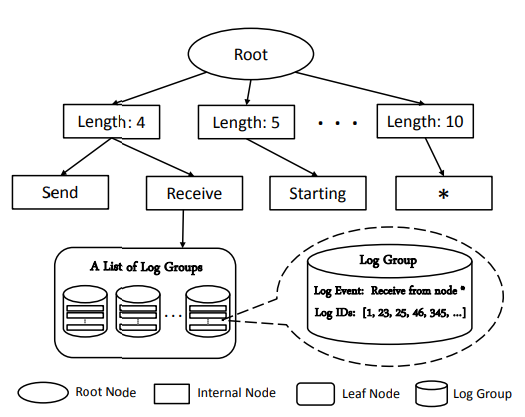
\includegraphics[scale=.5]{img/parse-tree-drain.PNG}}
            \caption{Structure of a simple parsing tree of depth $3$ in Drain \cite{drain2017}}
            \label{parseTreeDrain}
        \end{figure}
        
    The algorithm consists of five steps: 
    
    \begin{enumerate}
        \item \textit{Preprocess by Domain Knowledge}. According to empirical study on log parsing methods by He et al. \cite{logParsingEvaluation2016}, preprocessing improves parsing accuracy. Thus, when a new raw log message arrives, before constructing actual parse tree, Drain will preprocess it using regular expressions provided by user based on domain knowledge. This may include frequently used variables, e.g. IP address, and any matched tokens will be removed. 
        \item \textit{Search by Log Message Length}. In the next step, the parsing tree is being built. The process is based on the assumption that log messages with the same log event may have the same log message length. Starting from the root node, each node in the first layer represents log groups, whose log messages are of different length. The length of the message is specified by the number of tokens. Cases where log messages with the same log event have different lengths can be handled by postprocessing. For example, the path to preprocessed log message \texttt{Packet has been sent} to a first layer node would be \textit{Length: 4}.
        
        \item \textit{Search by Preceding Tokens}. In the third step, the parsing tree is traversed to a leaf node in the second layer. The assumption made in this step is that the first tokens in a log message are likely to be constants. For example, in the log message \texttt{Packet has been sent}, tree is traversed from first layer node \textit{Length: 4} to the leaf node with internal node \textit{Packet}, as "Packet" is considered to be a constant. Therefore, the second layer contains nodes with unique first words. Depending on the \textit{depth} of the tree, there is more internal nodes which search by the tokens in the first, second, third... etc. position. However, sometimes a variable word may appear in the beginning positions, such as \texttt{120 bytes received}. This is solved by only considering tokens that do not contain digits. If a token contains a digit, it matches a special internal node \textit{"*"}. 
        
        \item \textit{Search by Token Similarity}. After step 3, lists of log groups are contained in leaf nodes. Each log group has \textit{log event} and
\textit{log IDs}. Log event is the template describing the log messages of the group and log IDs are the log IDs of the log messages in that group. Each log group contains log messages of same length starting with the same word. In this step, Drain will calculate the similarity between the log message and the log event of each log group. Similarity is calculated over each token position. The highest similarity score is compared with a predefined similarity threshold, that indicates if the given log group is suitable.
        
        \item \textit{Update the Parse Tree}. In the final step, the log ID of the current log message is added to the most suitable log group from step $4$ and log event in the log group is updated (different tokens will be substituted by wildcard *). 
    \end{enumerate}

    \subsection{Summary} \label{parser_summary}
    In this section we presented an overview of automated log parsing techniques and their representative tools. Table \ref{tab:logParsers} provides a summary of all log parsing tools that we reviewed in this paper. The tools are compared from various aspects that we considered important for our use case. \textbf{Mode} denotes online or offline manner, while \textbf{Method} denotes the log parsing technique employed by the tool. \textbf{Preprocessing} describes if a extra manual preprocessing step is required. \textbf{Performance} categorizes tools into three levels based on their efficiency: high, medium and low, as suggested in \cite{zhlhxzl2018}. Lastly, having log parsing tools freely available is of huge importance for practical use. Therefore, the last column is dedicated to the \textbf{Open Source} characteristics of existing tool. 
    
    \begin{table}[t]
    \centering
    \resizebox{\textwidth}{!}{\begin{tabular}{|c|c|c|c|c|c|c|}
    \hline
    \textbf{Log Parsing Tool} & \textbf{Year} & \textbf{Mode} & \textbf{Method}         & \textbf{Preprocessing} & \textbf{Performance} &  \textbf{Open Source} \\ \hline
    SLCT             & 2003 & Offline & Frequent Pattern Mining & \xmark     & High     & \cmark         \\
    LogSig           & 2011 & Offline & Clustering              & \xmark      & Medium       & \xmark           \\
    IPLoM            & 2012 & Offline & Iterative Partitioning  & \xmark     & High        & \xmark           \\
    Drain            & 2017 & Online  & Fixed-depth tree        & \cmark    & High     & \cmark         \\ \hline
    \end{tabular}}
    \caption{Summary of automated log parsing tools}
    \label{tab:logParsers}
    \end{table} 
    
    After understanding and comparing the characteristics of different log parsing tools described in this section, as well as detailed evaluation of these tools on various systems in the paper by Zhu et al. \cite{zhlhxzl2018}, we chose Drain. The benchmarking results have shown that Drain is superior in terms of accuracy, robustness, and efficiency. In addition, its online character is of huge practical importance for our research, considering that Motorola SmartConnect system is constantly subject to changes. Also, we often work with smaller time intervals of data, therefore log lines generated in different time windows may lead to different event template set. Not having to provide the whole log data set before parsing is an undeniable advantage.
